\RequirePackage{luatex85}
\documentclass[tikz, border=10pt]{standalone}

\usepackage[compat=1.1.0]{tikz-feynman}

\begin{document}

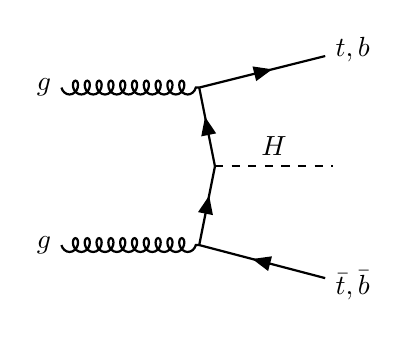
\begin{tikzpicture}[thick]
 \begin{feynman}
  \vertex (origin);
  \vertex [right=1.5cm of origin] (H);
  \vertex [above left=1cm and 0.2cm of origin] (v1);
  \vertex [below left=1cm and 0.2cm of origin] (v2);
  \vertex [left=1.75cm of v1] (g1) {\(g\)};
  \vertex [left=1.75cm of v2] (g2) {\(g\)};
  \vertex [above right=1.2cm and 1.4cm of origin] (t1) {\(t,b\)};
  \vertex [below right=1.2cm and 1.4cm of origin] (t2) {\(\bar{t},\bar{b}\)};
  \diagram* {
  (g1) -- [gluon] (v1),
  (g2) -- [gluon] (v2),
  (origin) -- [scalar, edge label={\(H\)}] (H),
  (origin) -- [fermion] (v1) -- [fermion] (t1),
  (t2) -- [fermion] (v2) -- [fermion] (origin),
  };
 \end{feynman}
\end{tikzpicture}
\end{document}
